% !TEX TS-program = pdflatex
% !TEX encoding = UTF-8 Unicode
% !TEX root = ../main.tex
% !TEX spellcheck = en-US
% ****************************************************************************************
% File: purpose_and_scope.tex
% Author: Patrick Haselwanter
% Date: 2023-10-28
% ****************************************************************************************
\chapter{Purpose and scope of the project}
\label{chapter:purpose_and_scope}
This report aims to summarize the used methods for implementing a state feedback control of an aerodynamic levitation system in the context of the course advanced control engineering. In this report, 
\begin{itemize}
    \item the methods used to identify the real system,
    \item the methods to design a suitable controller
    \item the validation of the controller through simulation 
    \item the methods used to implement the controller with the real hardware and
    \item the results of the real hardware implementation
\end{itemize}
    are described. The goal of this report is to summarize all information needed to be able to redo the lab task by an other person. 

\section{Introduction}



    \begin{figure}[h]   
    \centering
    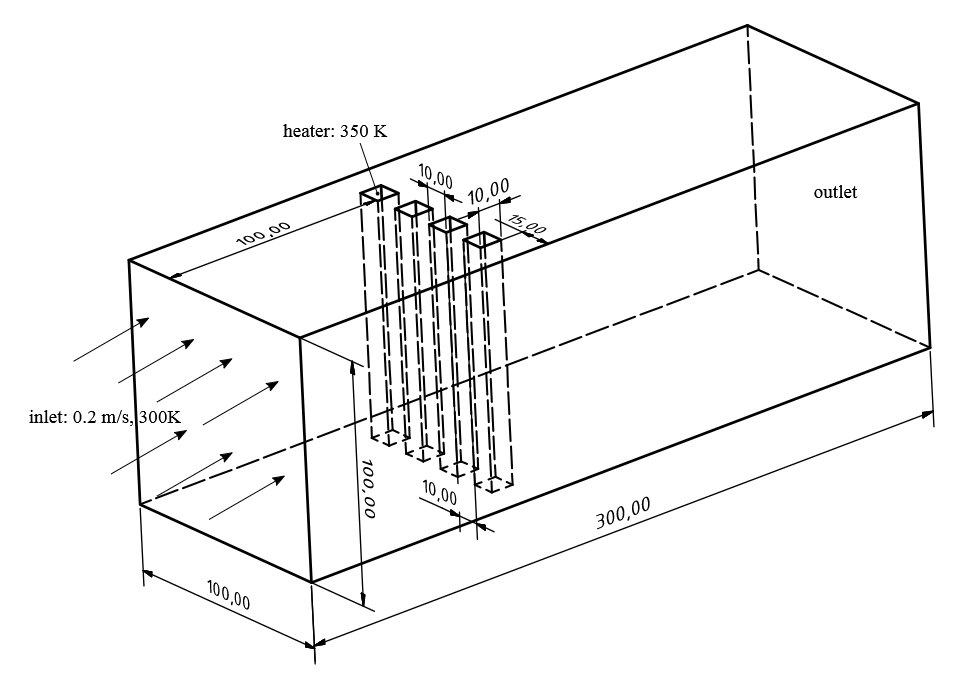
\includegraphics[width=0.7\textwidth]{img/heater_geo_og.png}
    \caption{Given heater geometry}
    \label{fig:heater_geo}
\end{figure}
% EOF
